\chapter[Adaptive User Scheduling]{Adaptive Block Diagonalization and User
Scheduling With Out of Cluster Interference\footnote{The work shown in this
chapter has been presented in \cite{jjgarcia14}.}}\label{ch:adaptive_schedule}

% ------------------------------------------------------------------------------
\section{Introduction}\label{sec:sched_intro}

In \refc{ch:achiev_rates} and \ref{ch:rate_statistics} the performance of a
clustered network using \gls{bd} has been analyzed, both in terms of mean
achievable rate per user and in terms of network fairness. In both studies, a
common result appears: a limited cluster size can be beneficial. This is true
not only regarding the rate that the users can achieve, but also considering
the requirements imposed on the network infrastructure. When the size of the
cellular network grows, global coordination becomes impractical, due to the
increased feedback and backhaul requirements. Additionally, there are
theoretical works that show how the gains from coordination are intrinsically
limited for an increasing network size \cite{lozano13}.

The main drawback of clustering is the presence of \gls{oci}, and in particular
\gls{bd} performs poorly when \gls{oci} is considered \cite{shim08}. The problem
approached in this chapter is the performance loss of \gls{bd} when \gls{oci} is
present. A simple and practical algorithm is presented, based on a hybrid
strategy combining \gls{bd} and \gls{su} processing. The best transmission
strategy is chosen according to a metric that is compared with a simple
threshold at each user equipment.

The scenario here considered is a multiuser network, with each cell serving
multiple users. A low-complexity algorithm is proposed to schedule the users,
trying to take advantage of the multiuser diversity to increase the mean rate
per user. In \cite{shen06} a similar suboptimal algorithm, based on the
Frobenius norm of the channel matrix is proposed, but it is not analyzed in the
presence of \gls{oci} nor is it combined with a hybrid precoding strategy.

% ------------------------------------------------------------------------------
\section{System Model}\label{sec:sched_system_model}

The system model used in this chapter is the same as the clustered network model
in \refc{ch:achiev_rates}. It is focused on the downlink of a cellular network
with a set of $\B = \Bin \cup \Bout$ of cells, where $\Bin$ is the set of $M$
cells that form the cluster under study, $\Bout$ represents the set of
$\Minterf$ cells external to the cluster, and $\Bin \cap \Bout = \emptyset$.
Again, it will be considered that each user is associated to one and only one
\gls{bs}.

The signal received at the $i$-th user equipment is then given by

\begin{equation} \label{eq:yi_oci_present}
    y_i = \HH_i \Wtx_i \ss_i + \underbrace{\sum\limits_{\substack{j=1\\j\neq i}}
    ^{N} \HH_i \Wtx_j \ss_j}_{\text{Inner Interference}} +
    \underbrace{\sum\limits_{k \in \Bout} \Hbar_{ik} \xbar_k}_{\text{OCI}}
    + \nn_i
\end{equation}

\noindent
which is another way of writing \eqref{eq:rx_signal_user_interf} when external
interference is considered. $\Hbar_{ik} \in \C^{r \times t}$ is the channel
matrix from the $k$-th \gls{bs} outside the cluster to the $i$-th user in the
cluster, and $\xbar_k$ is the transmitted signal at the $k$-th \gls{bs} outside
the cluster.

Analogously to \eqref{eq:interf_plus_noise}, the interference and noise terms in
\eqref{eq:yi_oci_present} can be grouped together

\begin{equation} \label{eq:zi_hat}
    \zhat_i = \sum\limits_{\substack{j=1\\j\neq i}}^{N} \HH_i \Wtx_j \ss_j +
    \sum\limits_{k \in \Bout} \Hbar_{ik} \xbar_k + \nn_i.
\end{equation}

The ergodic rate obtained at the $i$-th receiver can then be written as

\begin{equation} \label{eq:rate_yi_oci}
    R_i = \log_2\left|\eye + \HH_i\Wtx_i\RR_{\ss_i}\WtxH_i\HH_i^H
    \RR_{\zhat_i}^{-1}\right|
\end{equation}

\noindent
where

\begin{equation} \label{eq:zhat_cov}
\begin{aligned}
    \RR_{\zhat_i} &= \E\left\{\zhat_i\zhat_i^H\right\} \\
    &= \sum\limits_{\substack{j=1\\j\neq i}}^{N} \HH_i \Wtx_j \RR_{\ss_j}
    \WtxH_j \HH_i^H + \sum\limits_{k \in \Bout} \Hbar_{ik} \RR_{\xbar_k} 
    \Hbar_{ik}^H + \sigma^2\eye
\end{aligned}
\end{equation}

\noindent
is the covariance matrix of the interference plus noise vector in
\eqref{eq:zi_hat}.

The rate expression \eqref{eq:rate_yi_oci} depends on the transmission strategy
used within the cells of the cluster, represented by the precoding matrix
$\Wtx_i$ for $i \in \Bin$. In the current work two transmission strategies are
considered:

\begin{itemize}
    \item Block Diagonalization.
    \item Single User Processing.
\end{itemize}

% ------------------------------------------------------------------------------
\section{Transmission Strategy} \label{ssec:sched_strategy}

% ------------------------------------------------------------------------------
\subsection{Block Diagonalization} \label{ssec:sched_bd}

\gls{bd} transmission strategy has been thoroughly described in \refs{sec:bd} in
the absence of interference coming from outside the cluster that is coordinated
using \gls{bd}.

In this work, \gls{oci} is considered, and in this case \gls{bd}
is not able to remove it, as the \glspl{bs} only coordinate to get rid of the
interference from within the cluster. As a result, the rate obtained when using
\gls{bd} is no longer given by \eqref{eq:bd_ergodic_capacity}, but the following
revised expression

\begin{equation} \label{eq:bd_rate_oci}
    R_{i}^{\text{BD}} = \log_2\left|\eye + \bLambdahat_i \RR_{\ss_i}
    \bLambdahat_i^H \left(\sum\limits_{k \in \Bout} \Hbar_{ik} \RR_{\xbar_k}
    \Hbar_{ik}^H + \sigma^2\eye\right)^{-1}\right|
\end{equation}

\noindent
where the additional term due to the \gls{oci} is present and $\RR_{\xbar_k} =
\E\left\{\xbar_k \xbar_k^H\right\} \in \C^{t \times t}$ is the covariance matrix
of the signal transmitted from the $k$-th \gls{bs} outside the cluster.

% ------------------------------------------------------------------------------
\subsection{Single User Processing} \label{ssec:sched_su}

The other transmission strategy that is considered in this work is Single User
processing. This is the case when no coordination is used, so that each \gls{bs}
serves only one user and, therefore, all the rest of \glspl{bs} are considered
interferers.

This translates into

\begin{equation} \label{eq:wtx_su}
    \Wtx_{ij} = \zero \forall j \neq i.
\end{equation}

The signal received at the $i$-th user can be written as

\begin{equation} \label{eq:yi_su}
    y_i = \HH_{ii}\xx_i + \underbrace{\sum\limits_{\ell \in \Bin \backslash
    \left\{i\right\}} \HH_{i\ell} \xx_{\ell}}_{\text{Inner Interference}} +
    \underbrace{\sum\limits_{k \in \Bout} \Hbar_{ik} \xbar_k}_{OCI} + \nn_i
\end{equation}

Provided \eqref{eq:yi_su}, if the \gls{svd} of the channel matrix $\HH_{ii}$ is
considered

\begin{equation} \label{eq:hi_svd}
    \HH_{ii} = \UU_i \Lambda_i \VV_i^H
\end{equation}

\noindent
then the following precoding matrix can be used in order to maximize the rate of
the $i$-th user \cite{telatar99}

\begin{equation} \label{eq:precod_su}
    \Wtx_{ii} = \VV_i
\end{equation}

\noindent
so that, using $\UU_i^H$ as the receive filter, the achievable rate becomes

\begin{equation} \label{eq:rate_su}
\begin{aligned}
    &R_i^{\text{SU}} = \\
    &\log_2\left|\eye + \bLambda_i \RR_{\ss_i} \bLambda_i^H \left(
    \sum\limits_{\ell \in \Bin \backslash \left\{i\right\}} \HH_{i\ell}
    \RR_{\xx_{\ell}} \HH_{i\ell}^H + \sum\limits_{k \in \Bout} \Hbar_{ik}
    \RR_{\xbar_k} \Hbar_{ik}^H + \sigma^2 \eye \right)^{-1} \right|
\end{aligned}
\end{equation}

% ------------------------------------------------------------------------------
\subsection{Transmission Strategy Selection} \label{ssec:sched_selection}

In \cite{zhang10} it is shown that the maximum capacity of a \gls{miso} downlink
channel can be reached using a combination of two transmission strategies, the
optimal \gls{mrt} and \gls{zfbf}. Based on this, \cite{moon13} presents a method
for the users to decide locally and individually the most convenient
transmission strategy from the two options presented in \cite{zhang10}. The way
to do this is through a threshold on the \gls{sinr}, and a closed form
expression for this threshold is provided in \cite{moon13}.

In \cite{zuleita09}, a similar result to that of \cite{zhang10} is presented for
the \gls{mimo} case, but the solution offered, apart from not having a closed
form expression, was based on sequentially solving a series of optimization
problems, which renders its applicability rather difficult.

In the current work, the same approach as in \cite{moon13} is followed. The
proposal is to use a metric that can be easily calculated at each receiver, and
to compare this metric with a fixed threshold locally at each user in order to
decide which transmission strategy to use.

Intuitively, \gls{bd} will perform better when the \gls{oci} is low, compared to
the power received from the \glspl{bs} in the cluster. Hence, the proposed
metric is

\begin{equation} \label{eq:metric}
   \theta_i =
   \frac{\sum\limits_{j \in \Bin} \Tr\left(\HH_{ij}\RR_{\xx_j}\HH_{ij}^H\right)}
   {\sum\limits_{k \in \Bout} \Tr\left(\Hbar_{ik}\RR_{\xbar_k}\Hbar_{ik}^H
   \right)}
\end{equation}

\noindent
which is the quotient of the power received from the \glspl{bs} in the cluster
and the power received from the \glspl{bs} outside the cluster.

After the metric is computed, it is compared with a fixed threshold
$\thetath$ for which there is no closed form expression. That is the
reason why the threshold considered in this work is calculated through
simulations and it is assumed to be known by all the users. The details of how
this threshold is calculated are given in \refs{sec:sched_performance}.

The decision about what transmission strategy to use is made locally by each
user. The $i$-th user compares the metric $\theta_i$ with the threshold
$\thetath$, and decides to use \gls{bd} if $\theta_i >
\thetath$, and choosen \gls{su} if $\theta_i \leq \thetath$.

All the users feed back their decissions to their \gls{bs}, and this information
is jointly used by the \glspl{bs} in the cluster to coordinate the scheduling of
the users and the transmission strategy used for each of them.

% ------------------------------------------------------------------------------
\section{Scheduling}\label{sec:sched_scheduling}

After the users have made their decision and fed it back to the \glspl{bs},
these will know which users are more suited to being served using \gls{bd} and
which ones using \gls{su}.

Analogously to \cite{moon13}, the users are grouped so that the transmission
strategy in all the \glspl{bs} is the same within a given transmission interval.
The motive for this was simplicity, in \cite{moon13}, whereas in this work it is
proposed to guarantee a good performance. This is so because users served with
\gls{bd} will experience a serious degradation in their rate if not all the
\glspl{bs} in the cluster coordinate, \ie some of the \glspl{bs} transmit to
their users using \gls{su} precoding.

Users that are better served using \gls{su} are indiferent to other users'
strategies, as no power control is considered or used, and all \glspl{bs} will
be transmitting at maximum power. On the other hand, when the transmission
strategy used is \gls{bd}, which users are selected in each cell is an important
operating decision. Depending on the channel matrices of each user, the \gls{bd}
process will result in a higher or a lower rate. The objective is, then, to
group the users from different cells so that a certain metric is maximized. In
particular, the metric used in this work will be related to the achievable
sum-rate.

In \cite{yoo06} a similar approach is proposed for a \gls{miso} scenario, where
users are scheduled for simultaneous transmission when their channel vectors are
as orthogonal as possible. In the \gls{mimo} case the channels are not vectors
but matrices, and the concept of orthogonal channels is not as clear as in
\cite{yoo06}. They propose, nonetheless, an extesion to their user selection
algorithm that can deal with multiantenna users, but it is not applicable here
because of the selection of \gls{bd} as precoder, instead of \gls{zfbf} as
transmission strategy.

The objective of the current work is to group \gls{bd} users so that the result
of the \gls{bd} precoding yields the maximum achievable sum-rate. Equivalently,
the users will be scheduled for transmission in groups of $M$, \ie one per cell,
so that the values of the diagonal of $\bLambdahat_i$ in \eqref{eq:bd_rate_oci}
are maximized.

Given a square matrix $\AA$, the following identity relating its trace with the
sum of its eigenvalues holds

\begin{equation} \label{eq:eig_trace}
    \Tr\left(\AA\right) = \Tr\left(\text{eig}\left(\AA\right)\right)
\end{equation}

\noindent
where $\text{eig}\left(\AA\right)$ is a diagonal matrix whose elements are the
eigenvalues of the matrix $\AA$.

Additionally, the Frobenius norm of a matrix $\AA$ is defined as

\begin{equation} \label{eq:frob_norm}
    \left\|\AA\right\|_F = \sqrt{\Tr\left(\AA\AA^H\right)}
\end{equation}

Combining \eqref{eq:eig_trace} and \eqref{eq:frob_norm}, the following relation
can be expressed

\begin{equation} \label{eq:eig_frob}
    \Tr\left(\text{eig}\left(\AA\AA^H\right)\right) = \left\|\AA\right\|_F^2
\end{equation}

\noindent
can be used to have a measure of the magnitude of the eigenvalues of the matrix
$\AA$, and it is a good candidate as metric to group the users for \gls{bd},
similarly to what is done in \cite{shen06}.

Given the $i$-th user's channel matrix $\HH_i$, in order to search for the user
$j$ that will yield the maximum sum-rate using \gls{bd}, the idea is to look for
the user $j$ with channel matrix $\HH_j$ that maximizes the Frobenius norm of
the compound matrix, because

\begin{equation} \label{eq:bd_frob}
    \Tr\left(\bLambdahat_{ij}\right) \propto \left\|\left[
    \begin{array}{c}\HH_i \\ \HH_j\end{array}\right]\right\|_F^2
\end{equation}

\begin{algorithm}[t]
\caption{BD User Selection}
\label{alg:bdus}
\begin{algorithmic}[1]
\State Sort the set $\Ubd$ in decreasing order of $\theta_i$
\While{$\lvert\Ubd\rvert \geq M$}
	\State $i = \first\left(\Ubd\right)$
	\State $\U_g = \left\{i\right\}$
	\State $\Ubd = \Ubd \backslash \left\{ i \right\}$
	\State $\HH_g = \HH_i$
	\State $N_g = 1$
	\While{$N_g \leq M$}
		\State $j = \argmax\limits_{j \in \Ubd \backslash \cell\left(\U_g\right)} \left\|\left[\begin{array}{c}\HH_g \\ \HH_j \end{array}\right]\right\|_F$
		\State $H_g = \left[\begin{array}{c}\HH_g \\ \HH_j \end{array}\right]$
		\State $N_g = N_g + 1$
		\State $\U_g = \U_g \cup \left\{j\right\}$
		\State $\Ubd = \Ubd \backslash \left\{ i \right\}$
	\EndWhile
\EndWhile
\end{algorithmic}
\end{algorithm}

\refal{alg:bdus} is proposed to form the groups of $M$ users that maximize the
rate using \gls{bd}. First the set of users that want to be served using
\gls{bd}, $\Ubd$, is sorted in descending order, with respect to the magnitude
of the metric \eqref{eq:metric}. Then the groups of $M$ users are generated by
adding one user at a time, using the Frobenius norm of the resulting matrix as a
measure of the magnitude of the singular values after performing the \gls{bd},
as suggested by \eqref{eq:bd_frob}.

In \refal{alg:bdus}, the functions \emph{first} and \emph{cell} refer to getting
the first element in an ordered set, and to returning the set of users in the
same cells as the users in the argument set, respectively. A possible result of
\refal{alg:bdus} is that not all the users that have selected \gls{bd} as their
preferred transmission strategy can be fit in a group with other \gls{bd} users.
In that case, the excess users are served using \gls{su}.

Finally, a round-robin strategy is used to transmit to all the groups that have
been formed, both the \gls{bd} and \gls{su} groups.

% ------------------------------------------------------------------------------
\section{Transmission strategy threshold computation}
\label{ssec:sched_threshold}

In \refs{sec:sched_scheduling} the threshold $\thetath$ was introduced as the
means for the users to decide between the two possible transmission strategies.
This threshold is assumed to be fixed, and it is precalculated via simulations.

In order to calculate the threshold a single user is placed in each of the cells
of the cluster, then the rate is calculated both when all the \gls{bs}
coordinate to transmit using \gls{bd} and when they transmit independently using
\gls{su}. Apart from the rate for the two transmission strategies, the metric in
\eqref{eq:metric} is also computed. This process is repeated for multiple user
locations and channel realizations.

\begin{figure}[t]
    \centering
    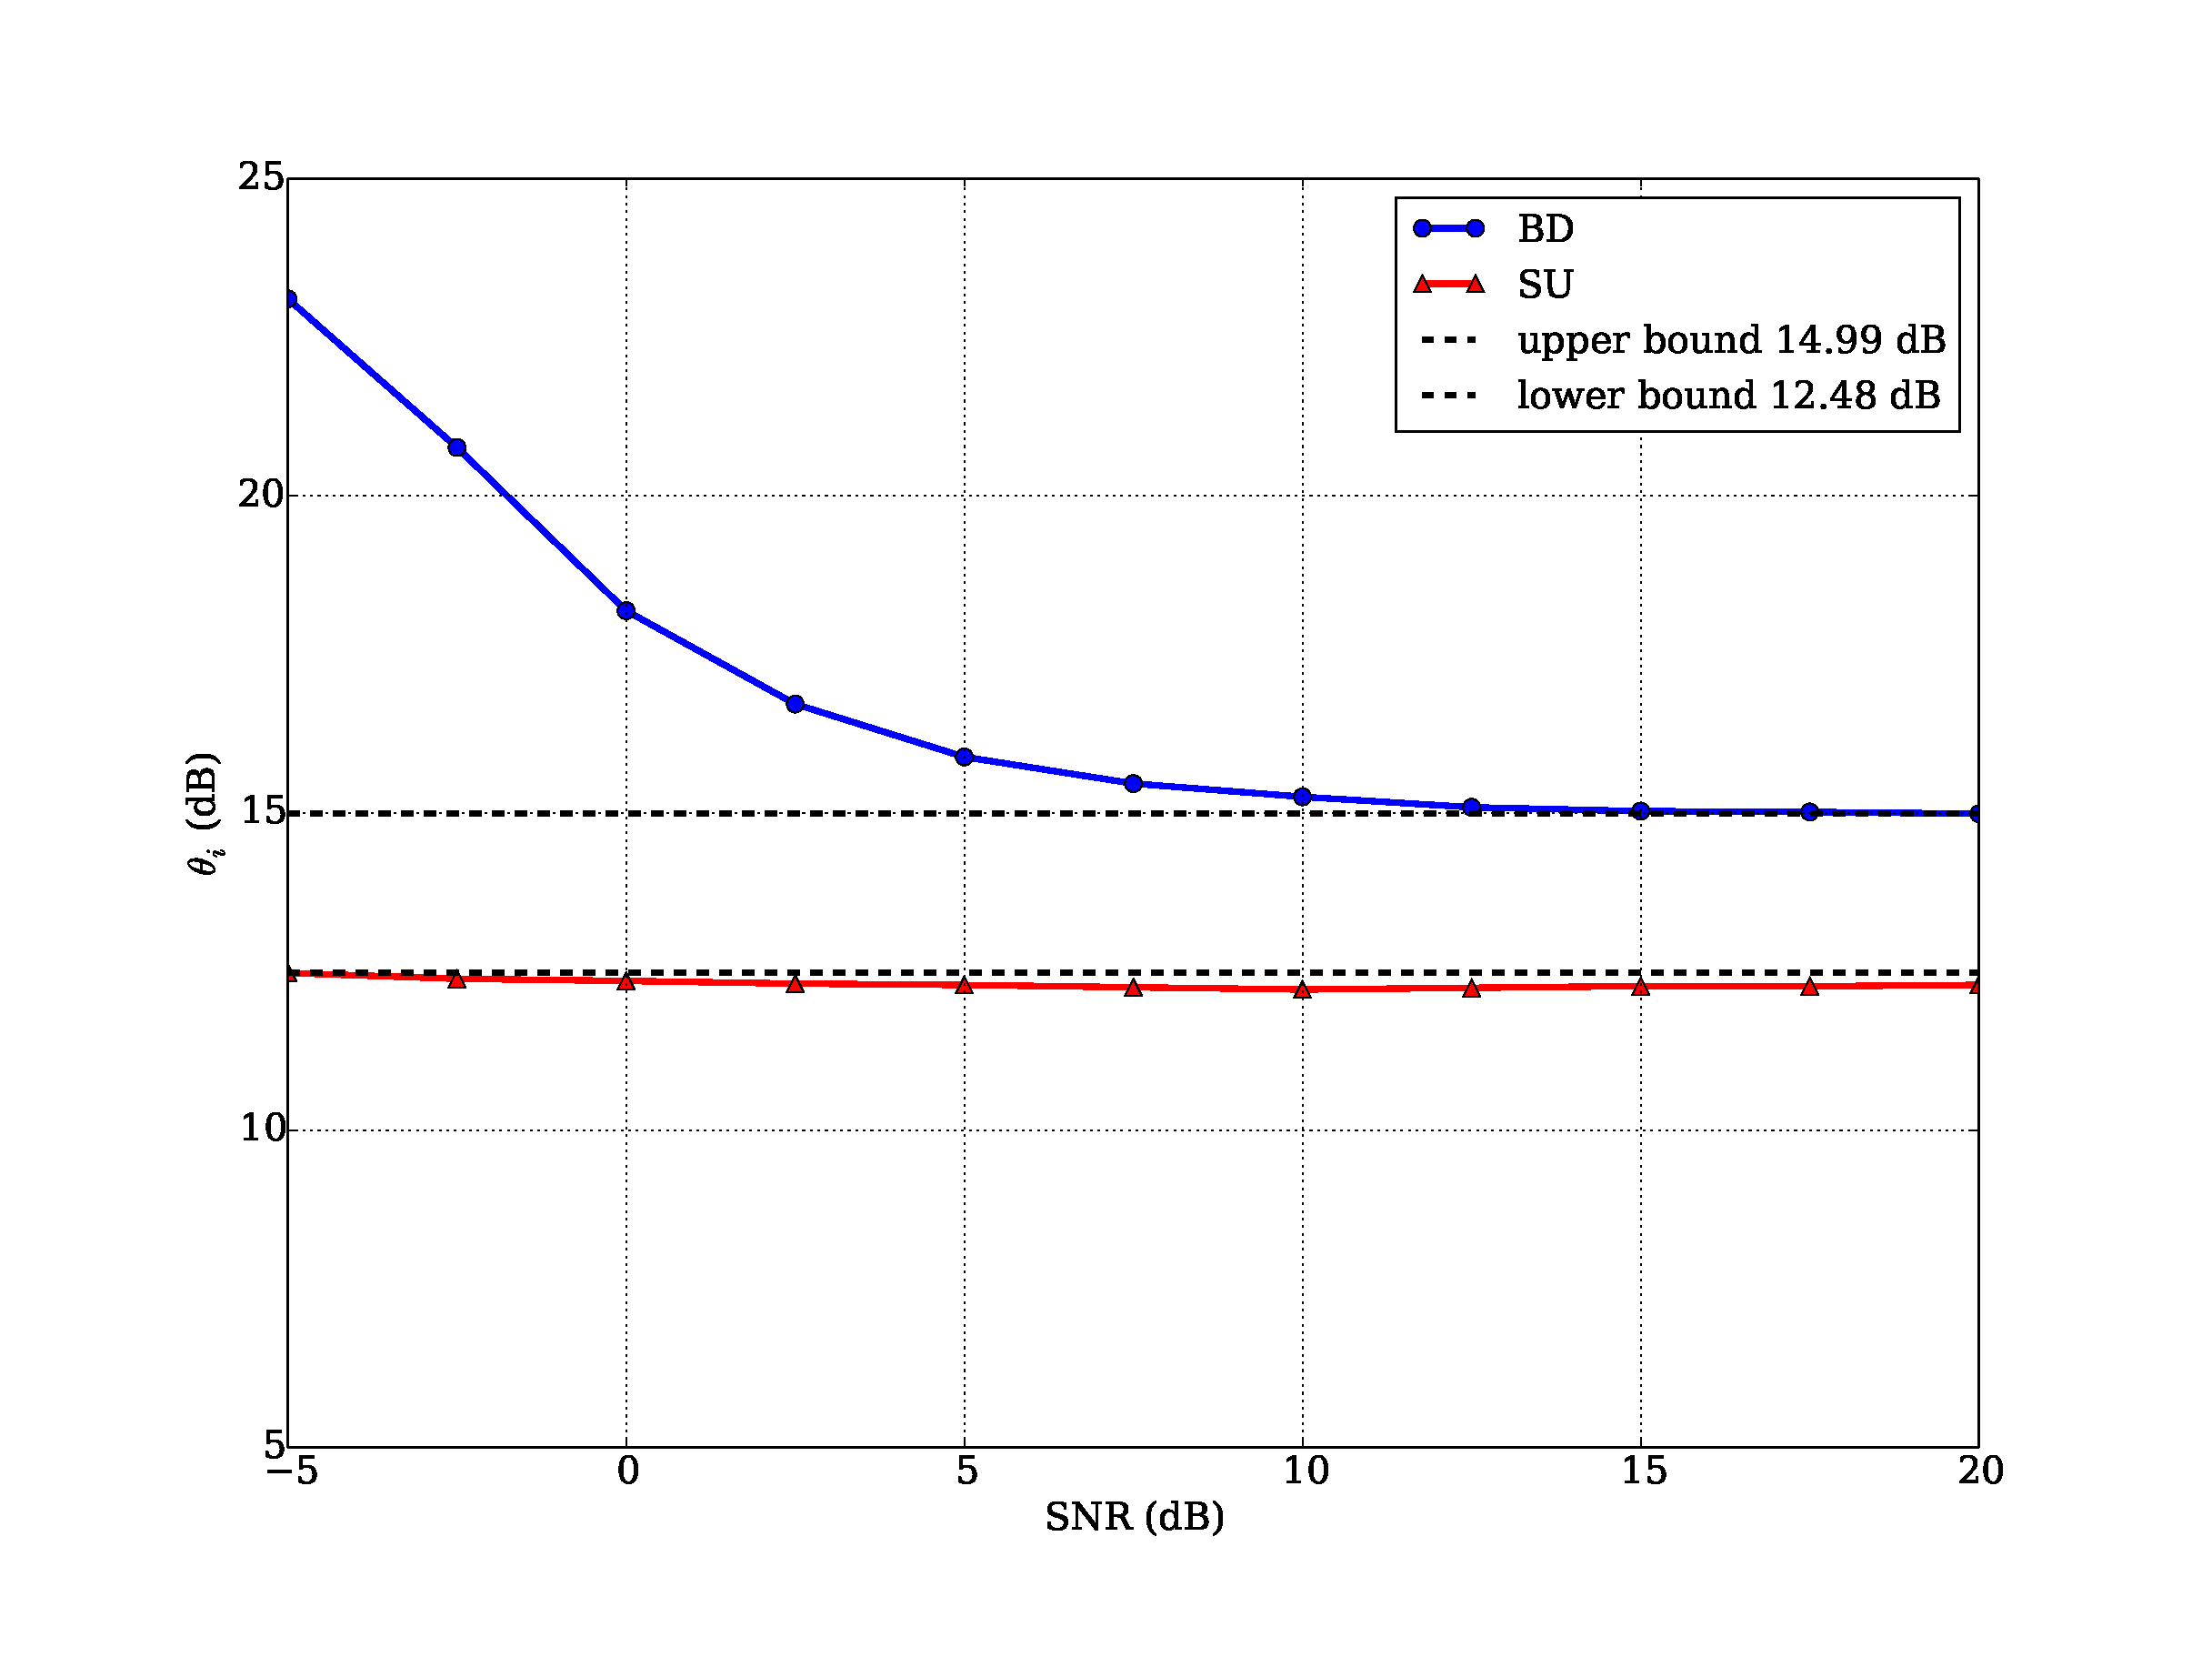
\includegraphics[width=0.75\columnwidth]{./12.simple_threshold_scheduling/img/mean_metric_02x02}
    \caption{Mean value of the metric for different \gls{snr} values, in the
    presence of \gls{oci} for a 7 cell cluster with 2x2 antennas configuration.}
    \label{fig:threshold_2x2}
\end{figure}

With the data gathered through the simulations described, it is possible to get
\reff{fig:threshold_2x2} where each of the solid curves represents the mean
value of the metric in \eqref{eq:metric}, in dB, for the users whose rate is
higher using \gls{bd} (blue), and for those who are better off being served
using \gls{su} (red). The dashed curves bound a gap between both curves, that
will be used to select the threshold $\phi_{\text{th}}$ for \eqref{eq:metric}.
For the example in \reff{fig:threshold_2x2}, the value chosen for the threshold
is the mean of the \emph{upper} and \emph{lower} bounds in the figure, yielding
a value of $\thetath = 13.74$\,dB.

As it has already been said, this value of the threshold is assumed to be fixed
and it has to be precomputed for the particular scenario under study.
\reff{fig:threshold_2x2} is calculated for the scenario represented in
\reff{fig:scenario_threshold}, which is also used in
\refs{sec:sched_performance} to asses the performance of the algorithm proposed
in this work.

\refa{ch:appendix_b} offers a characterization of the behavior of $\thetath$ for
different values of the scenario and system parameters, so that its dependence
on these factors can be observed.

% ------------------------------------------------------------------------------
\section{Performance Analysis}\label{sec:sched_performance}

The cellular scenario considered in this chapter differs slightly from the
scenario used in \refc{ch:achiev_rates} and \ref{ch:rate_statistics}. A single
cluster of 7 cells is considered, in a hexagonal layout and surrounded by a
single tier of cells that will account for the \gls{oci}.

\begin{figure}[t]
    \centering
    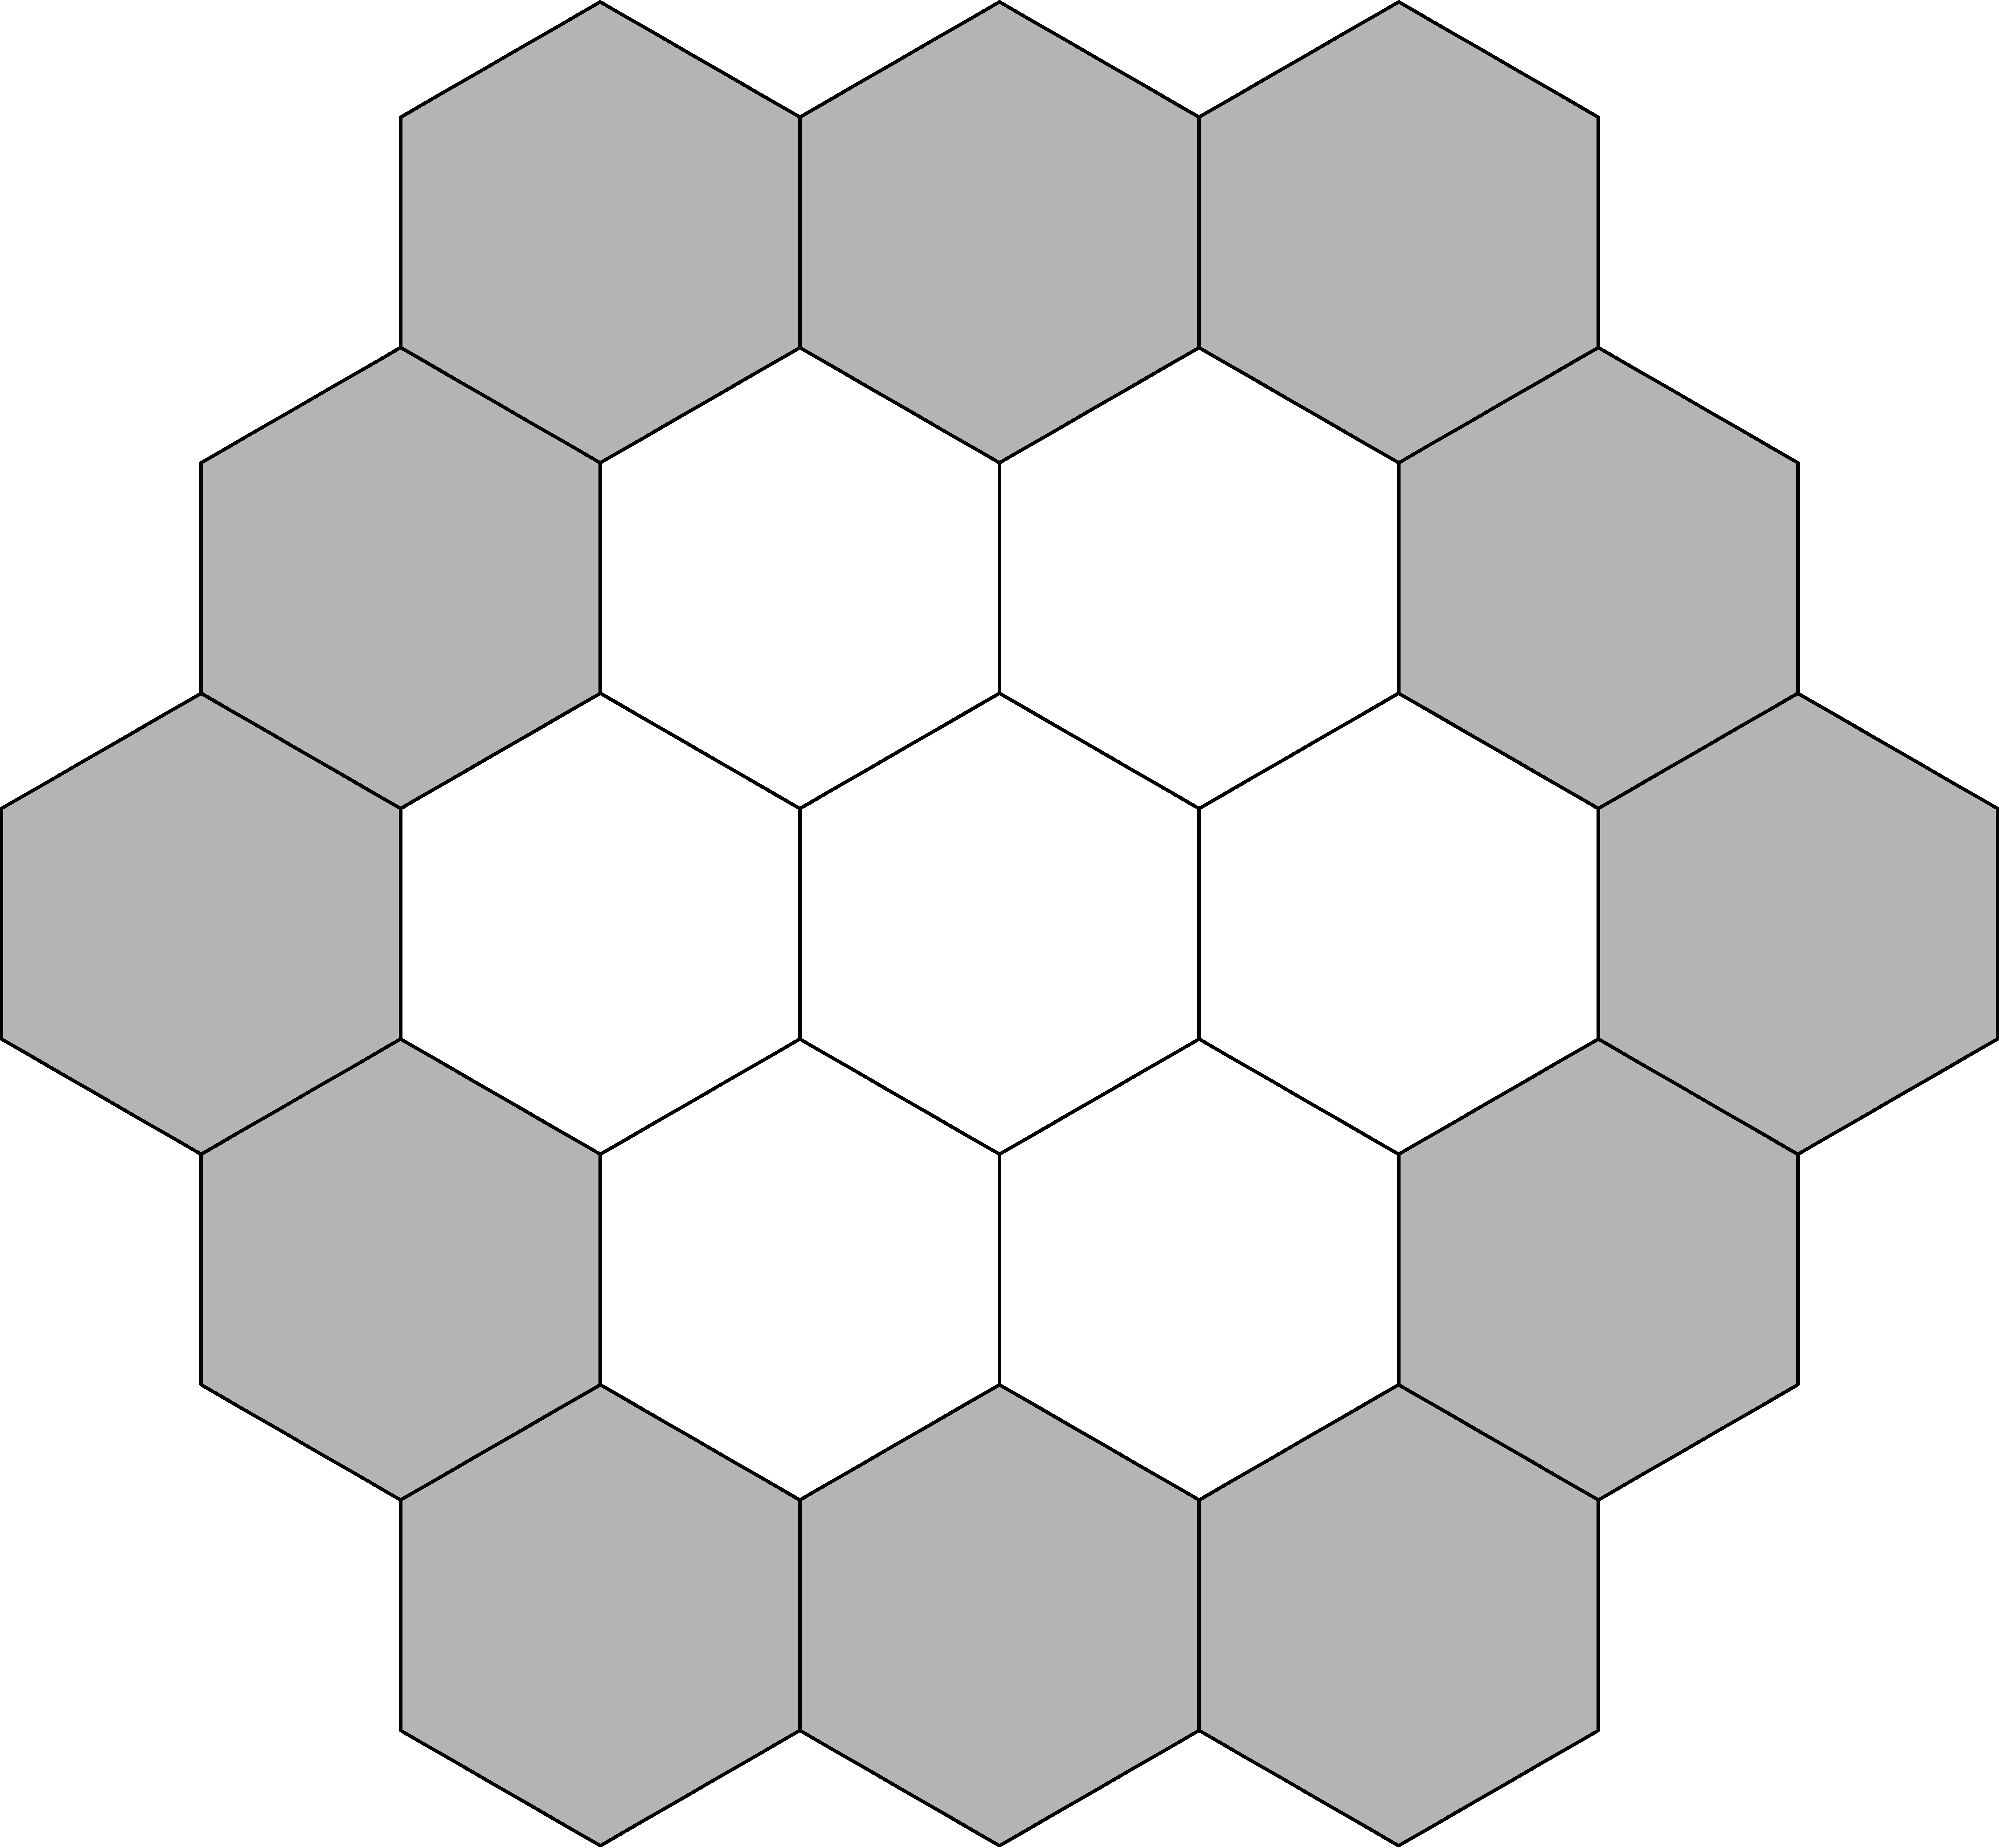
\includegraphics[width=0.75\columnwidth]{./12.simple_threshold_scheduling/img/scenario}
    \caption{The cells in the cluster (white) experience the \gls{oci} generated
    by the interfering cells (shaded).}
    \label{fig:scenario_threshold}
\end{figure}

\reff{fig:scenario_threshold} shows the scenario used in this chapter, where the
white cells form the cluster under study, and the shaded cells represent the out
of cluster interferers.

At each simulation run, 100 \gls{iid} users are randomly placed within each cell
of the cluster, according to a uniform spatial distribution over each cell. Each
of the users has the same antennas as each of the \glspl{bs}, \ie $t=r$, either
2 or 3 in the simulations.

The channel model used is described in \refs{sec:channel_model}.

After all the users are placed in the scenario, they are scheduled for
transmision and immediately after that the rate is calculated for the following
transmission options:

\begin{itemize}
    \item All \glspl{bs} transmit using \gls{su}.
    \item All \glspl{bs} transmit using \gls{bd}.
    \item The transmission strategy is chosen using the algorithm and scheduling
        proposed in this paper.
    \item The same as the previous, but the scheduling is performed based on the
        rates obtained using \gls{bd} instead of the approximation in
        \eqref{eq:bd_frob}.
\end{itemize}

In all cases, the power assignment is done using the scaled water-filling
described in \refss{ssec:scaled_wf}, in order to accomodate the \gls{pbpc}.

\begin{figure}[t]
\centering
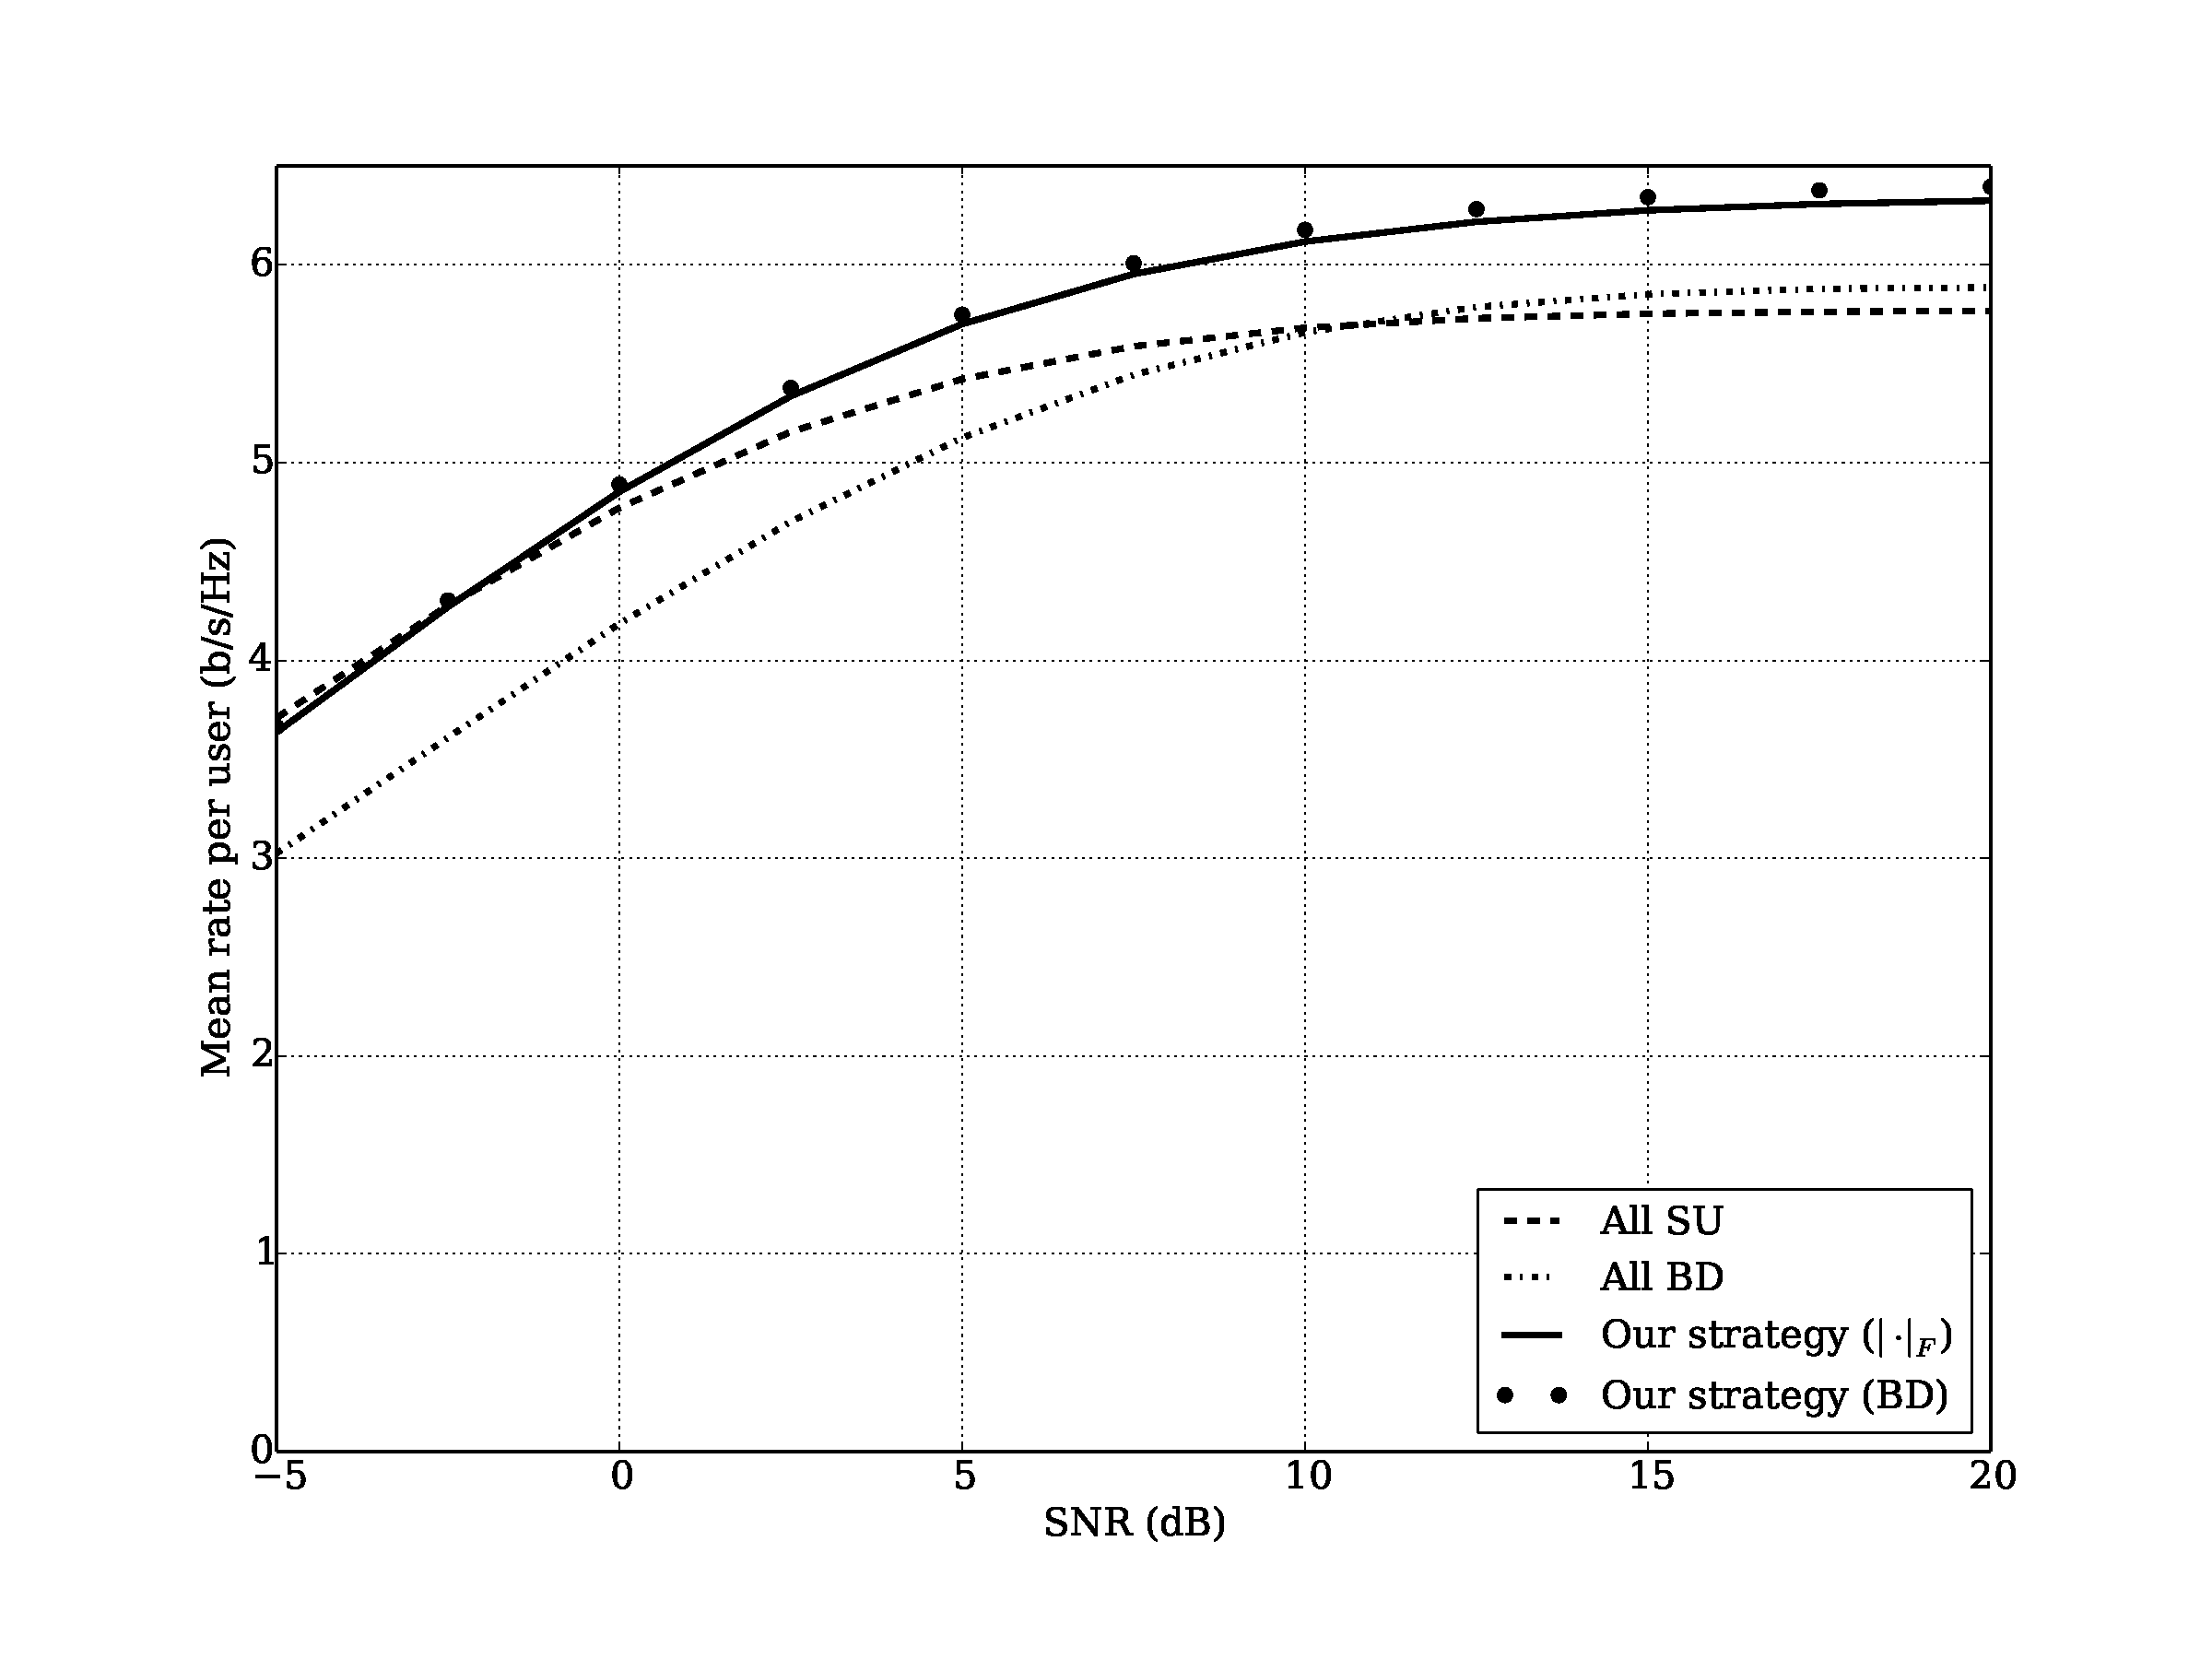
\includegraphics[width=0.75\columnwidth]{./12.simple_threshold_scheduling/img/mean_rate_02x02_100user_bd}
\caption{Mean rate obtained for a 2x2 scenario in the presence of \gls{oci}, 100
users per cell.}
\label{fig:mean_rate_2x2}
\end{figure}

\begin{figure}[t]
\centering
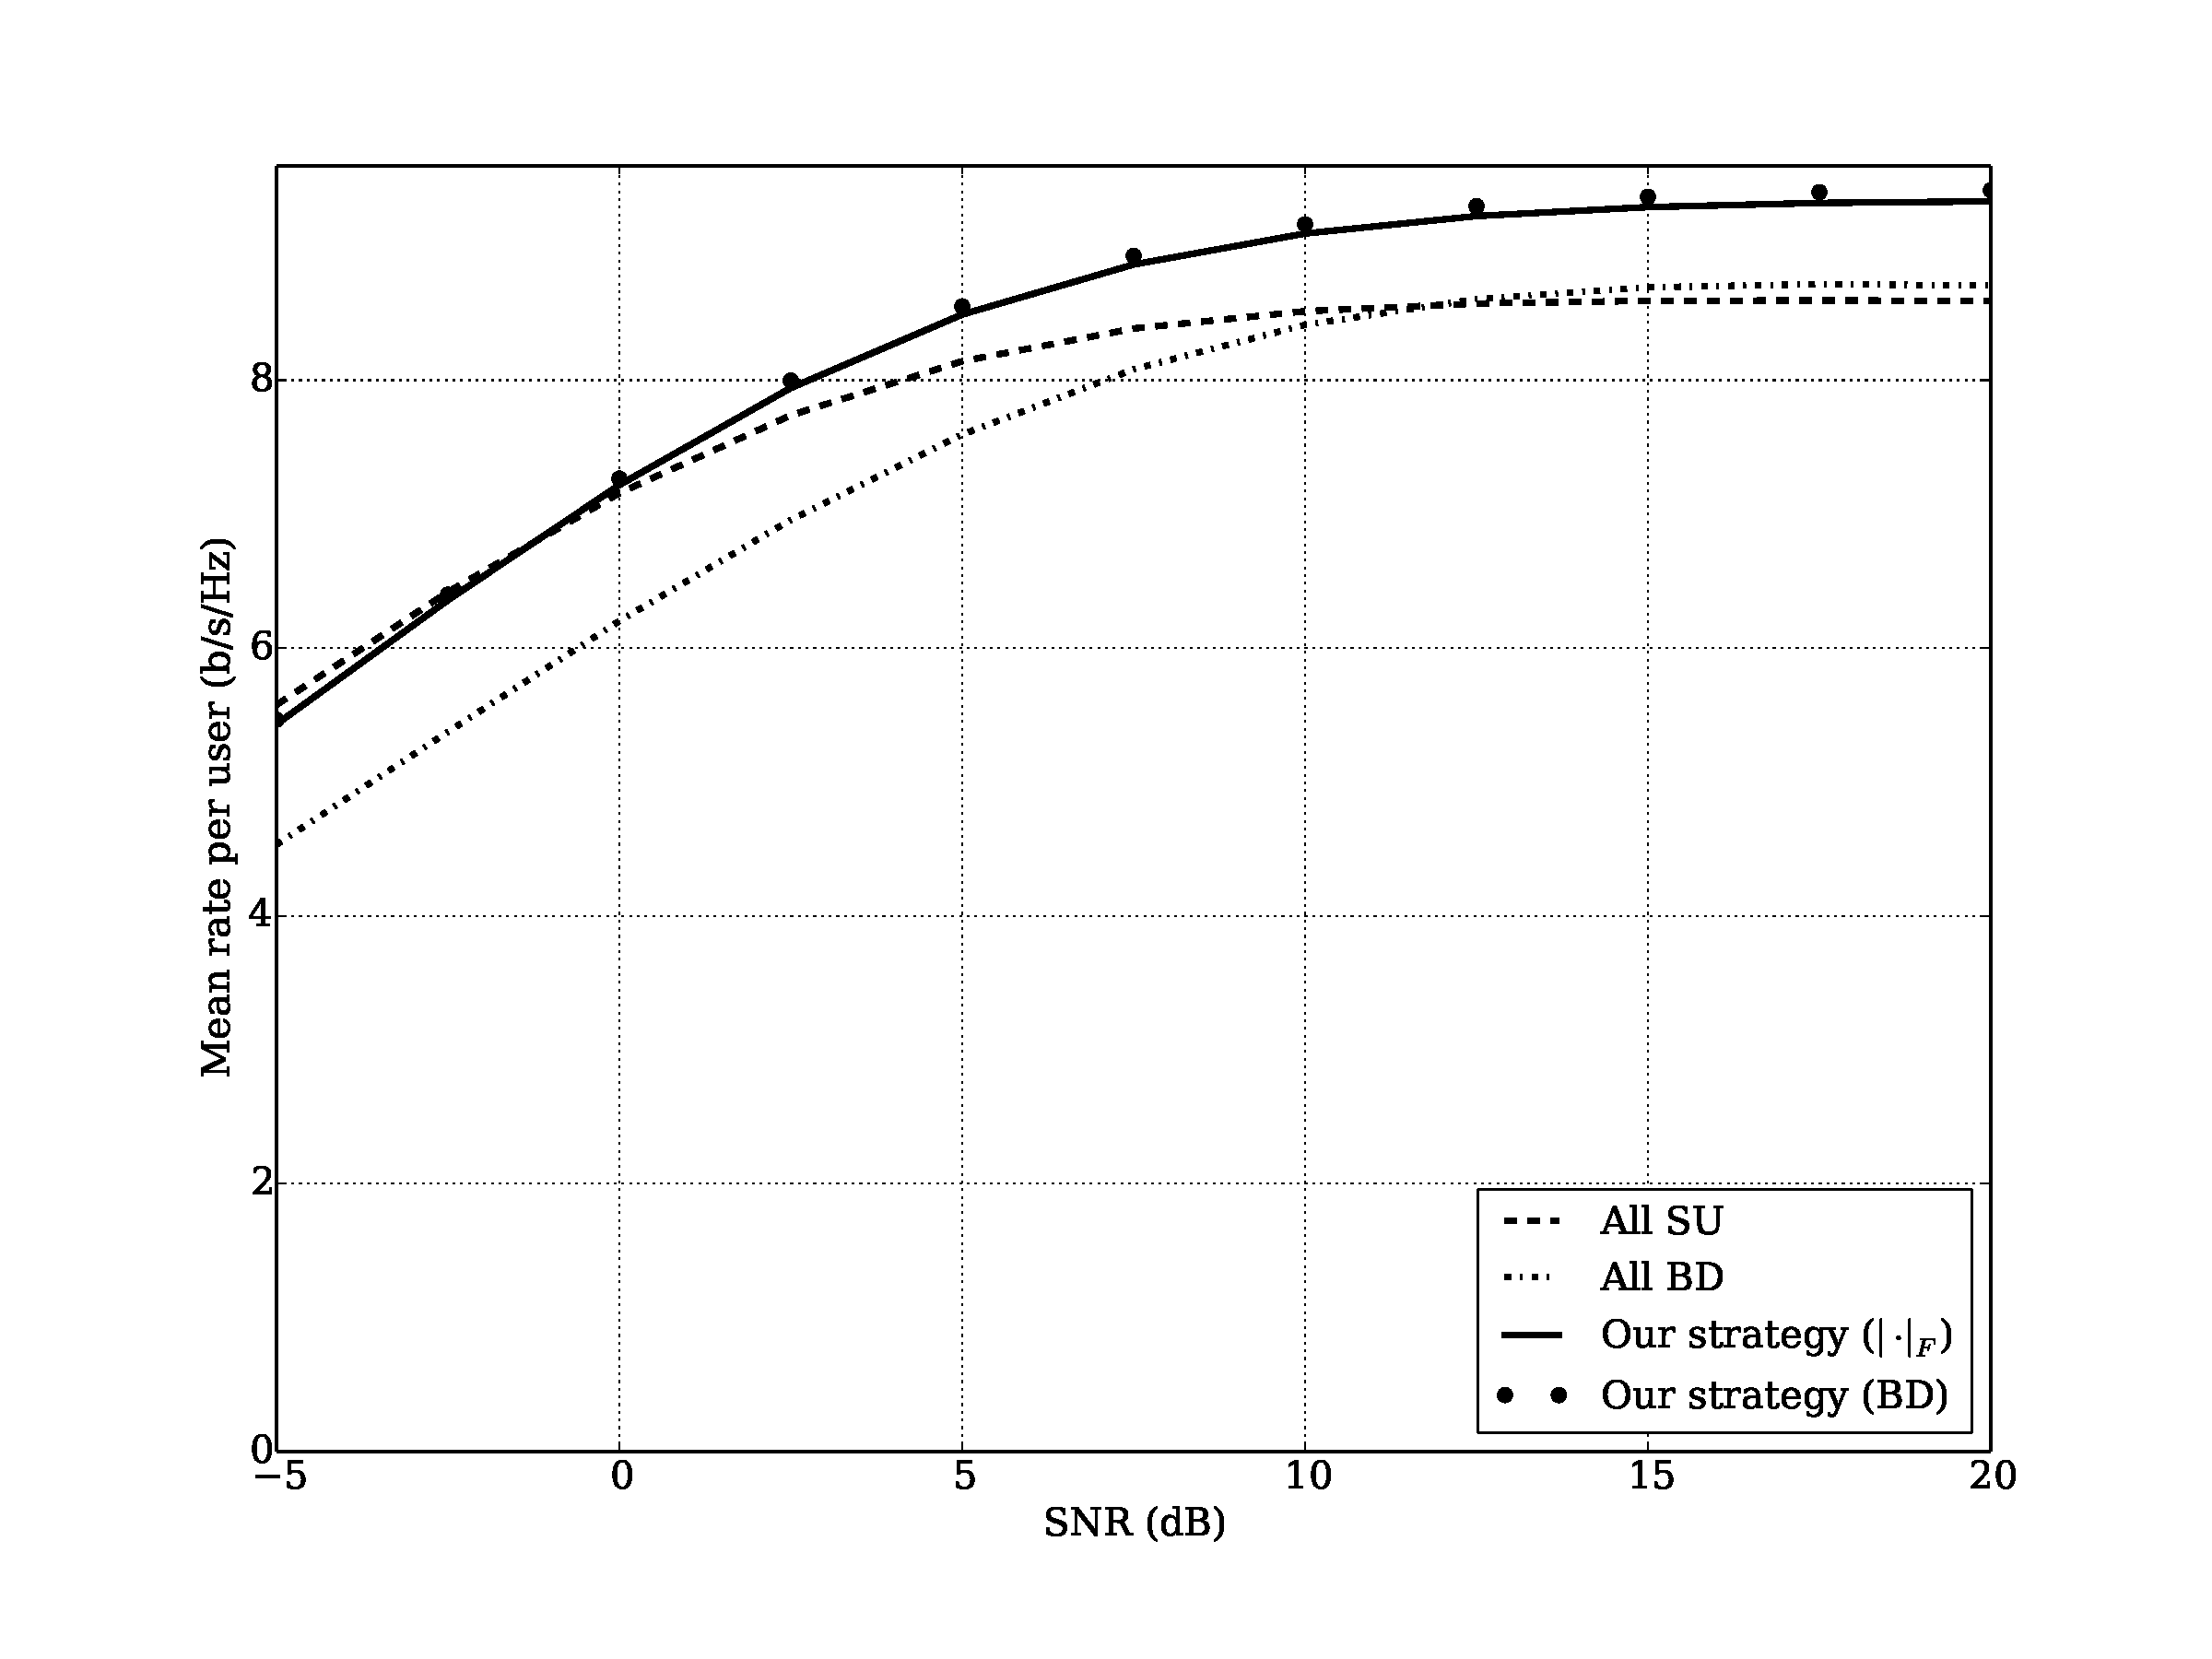
\includegraphics[width=0.75\columnwidth]{./12.simple_threshold_scheduling/img/mean_rate_03x03_100user_bd}
\caption{Mean rate obtained for a 3x3 scenario in the presence of \gls{oci}, 100
users per cell.}
\label{fig:mean_rate_3x3}
\end{figure}

\reff{fig:mean_rate_2x2} and \reff{fig:mean_rate_3x3} show the mean achievable
rate per user for the transmission options considered, and for two \gls{mimo}
configurations, $t=r=2$ and $t=r=3$ respectively. First thing that can be seen
is how the \gls{oci} severely degrades the performance of \gls{bd}, especially
in the low \gls{snr} regime, where it actually performs worse than not using
coordination at all. The user of the mixed strategy proposed in this work
improves the performance over the whole \gls{snr} range. It is important to note
how the approximation suggested in \eqref{eq:bd_frob} is highly accurate,
compared to using \gls{bd} to calculate the rates for the scheduling algorithm.
And not only is it accurate, but it also is much simpler to implement and much
less computationally expensive
\footnote{As described in \refc{ch:system_model} the \gls{bd} computation
involves two \gls{svd}, which has an overall computational complexity of
$O\left(mn^2\right)$ for a matrix of dimmensions $m \times n$,
\cite{golub2012matrix}. In contrast the computation of Frobenius norm, which
essentially requires the addition of all the elements of a matrix, with a
complexity of $O\left(mn\right)$.}

\begin{figure}[t]
\centering
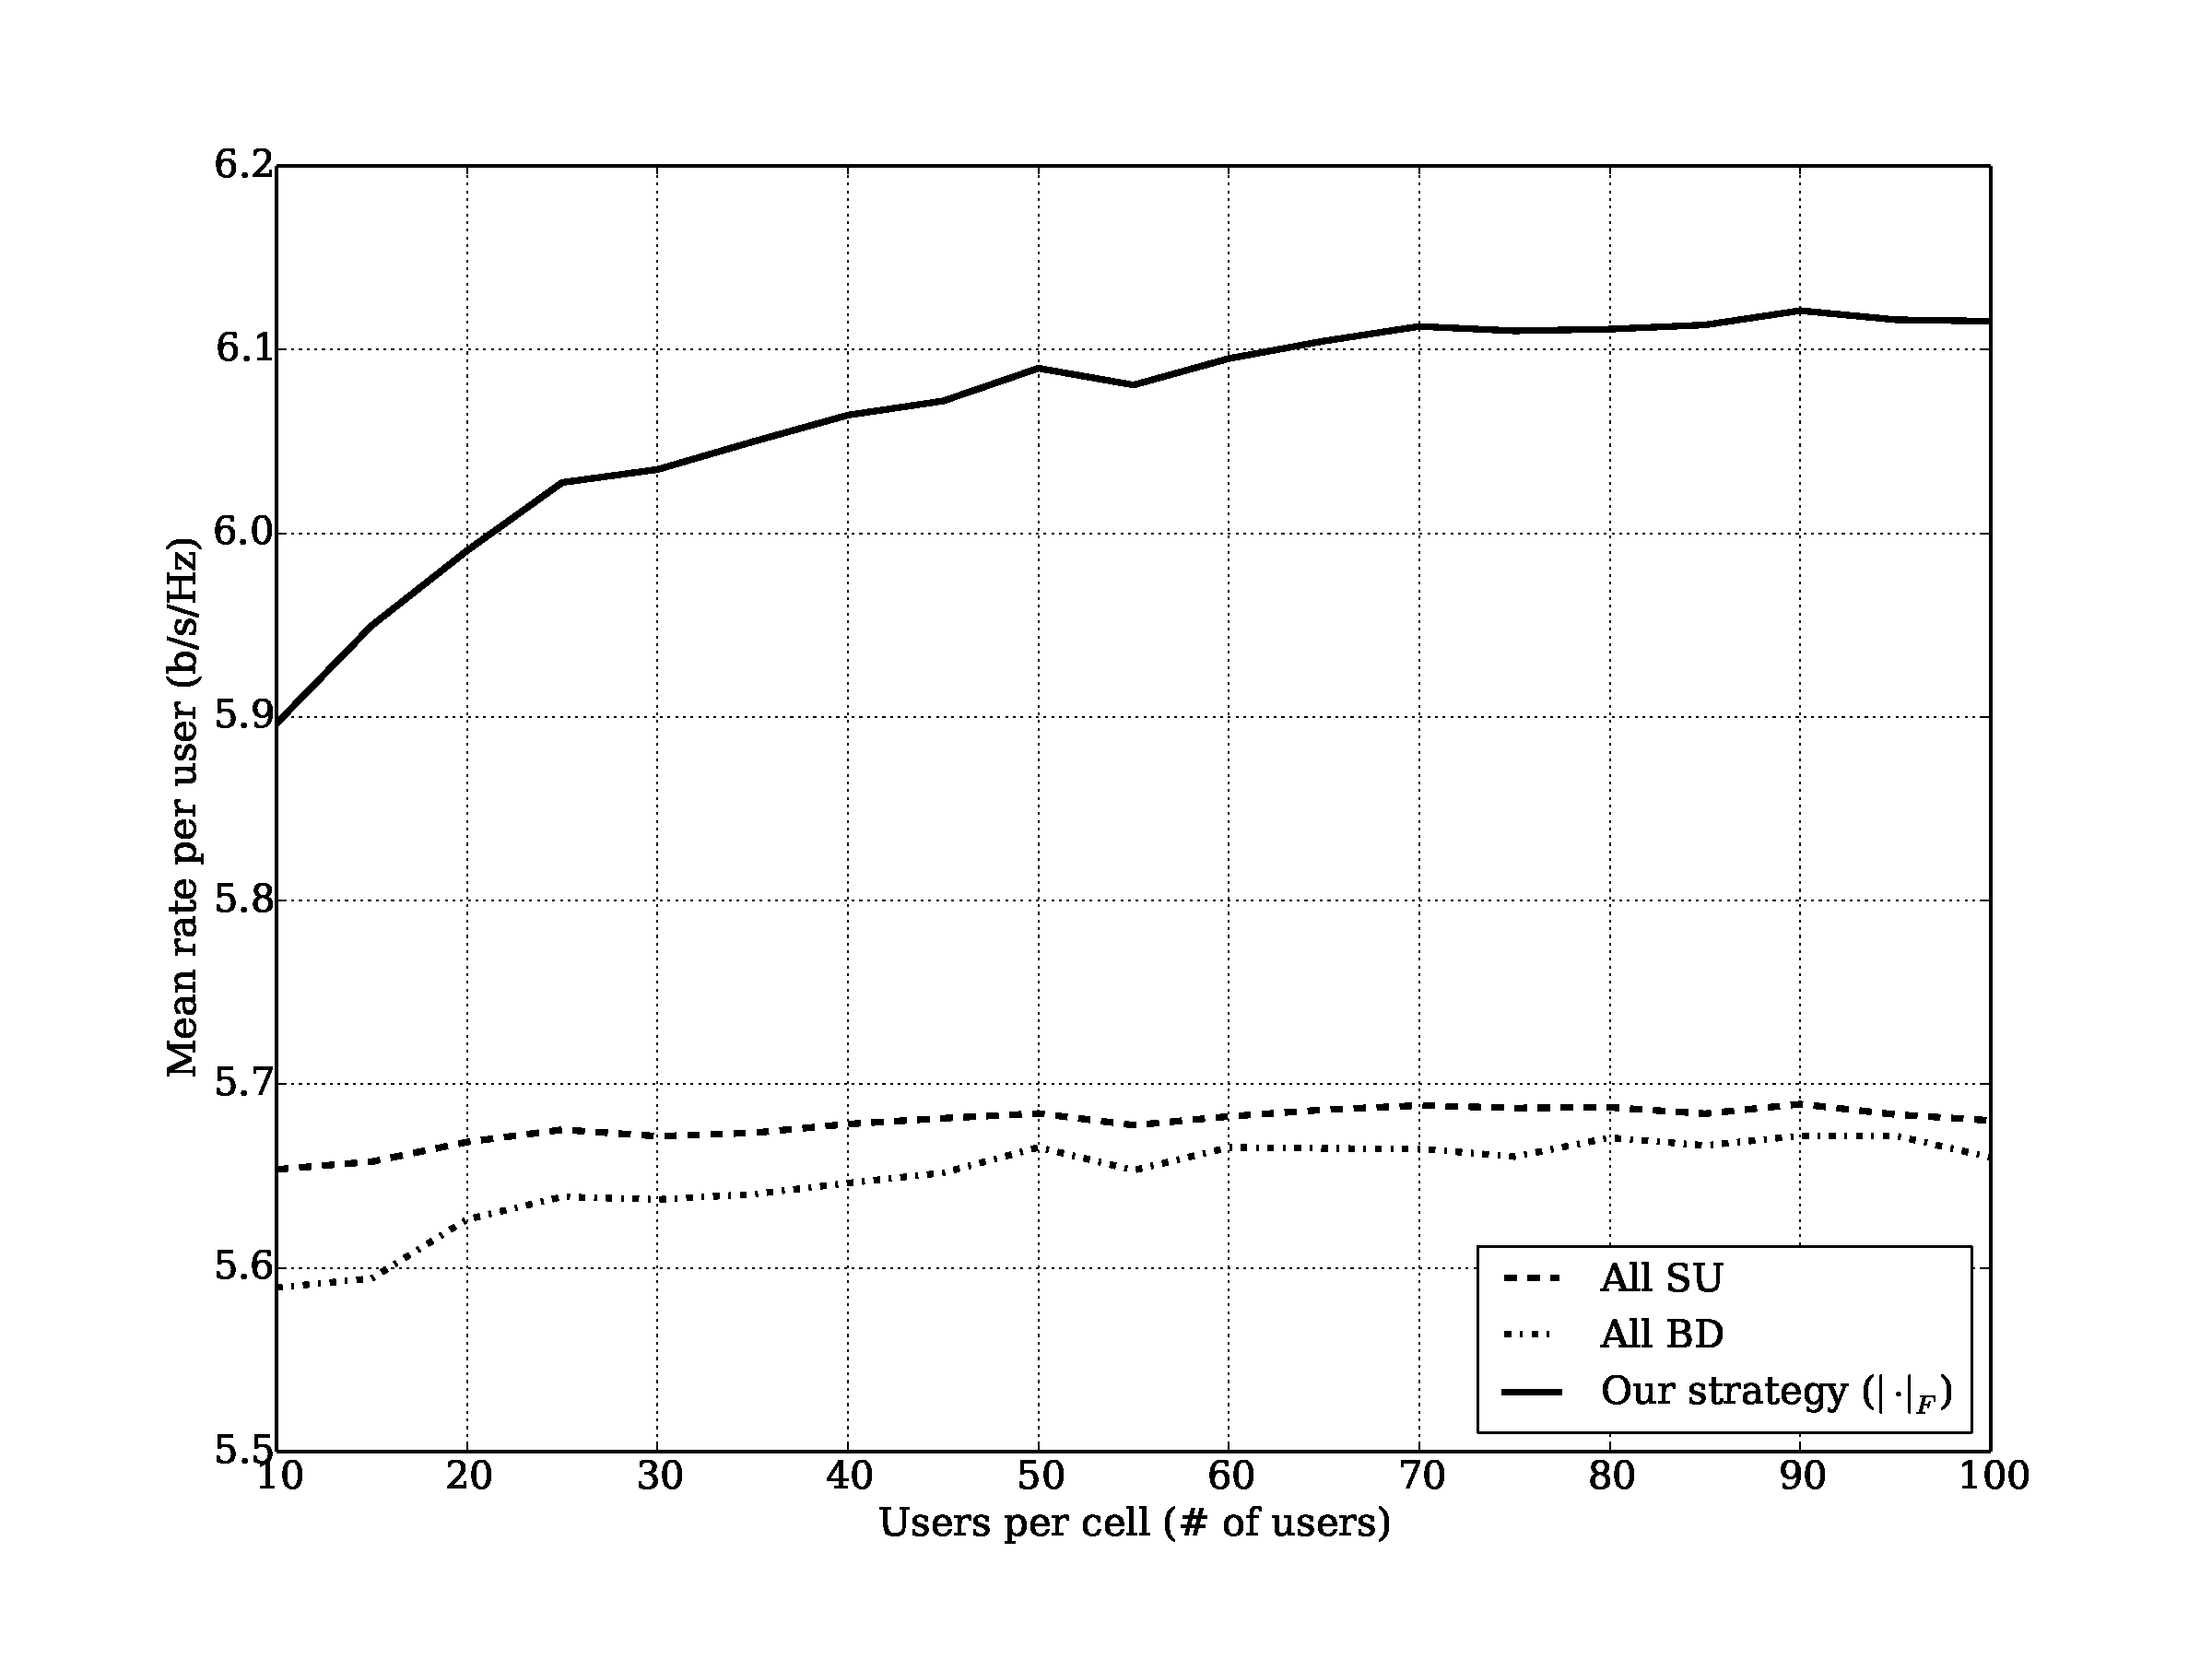
\includegraphics[width=0.75\columnwidth]{./12.simple_threshold_scheduling/img/mean_rate_vs_users_02x02_s10}
\caption{Mean rate for a 2x2 scenario as a function of the number of users per cell, for an SNR of 10\,dB.}
\label{fig:mean_rate_vs_users}
\end{figure}

In \reff{fig:mean_rate_vs_users} the mean achievable rate per user is presented as a function of the number of users per cell, for a fixed value of \gls{snr} of
10\,dB. The improvement introduced by the proposed scheme with respect to both
\gls{bd} and \gls{su} increases with the number of users per cell. This is easy
to explain, as the more users there are in each cell, the increased multiuser 
diversity makes it more likely to find the right users to form a group.

It is clear, from the previous results, that the \gls{oci} has a very serious
impact on the performance of \gls{bd}, but this is even more severe when the
fairness of the rates of all users is considered. \reff{fig:cdf_snr10}
represents the \gls{cdf} of the rates obtained with each of the transmission
strategies for a fixed value of \gls{snr} of 10\,dB. It can be seen how the
rates obtained using the mixed strategy are always higher than using each of the
strategies, \gls{bd} or \gls{su}, independently. This difference in favor of the
mixed strategy is even higher for the users with the lowest rates, which
indicates an improvement in the fairness of the system.

\reff{fig:worst_rate} shows the average rate for the 5\,\% worst users. For
these users, \gls{bd} in the presence of \gls{oci} performs poorly, and the use
of the hybrid strategy proposed in this work allows to recover from the loss due
to the \gls{oci}, and to match the performance obtained using \gls{su}.

\begin{figure}[t]
\centering
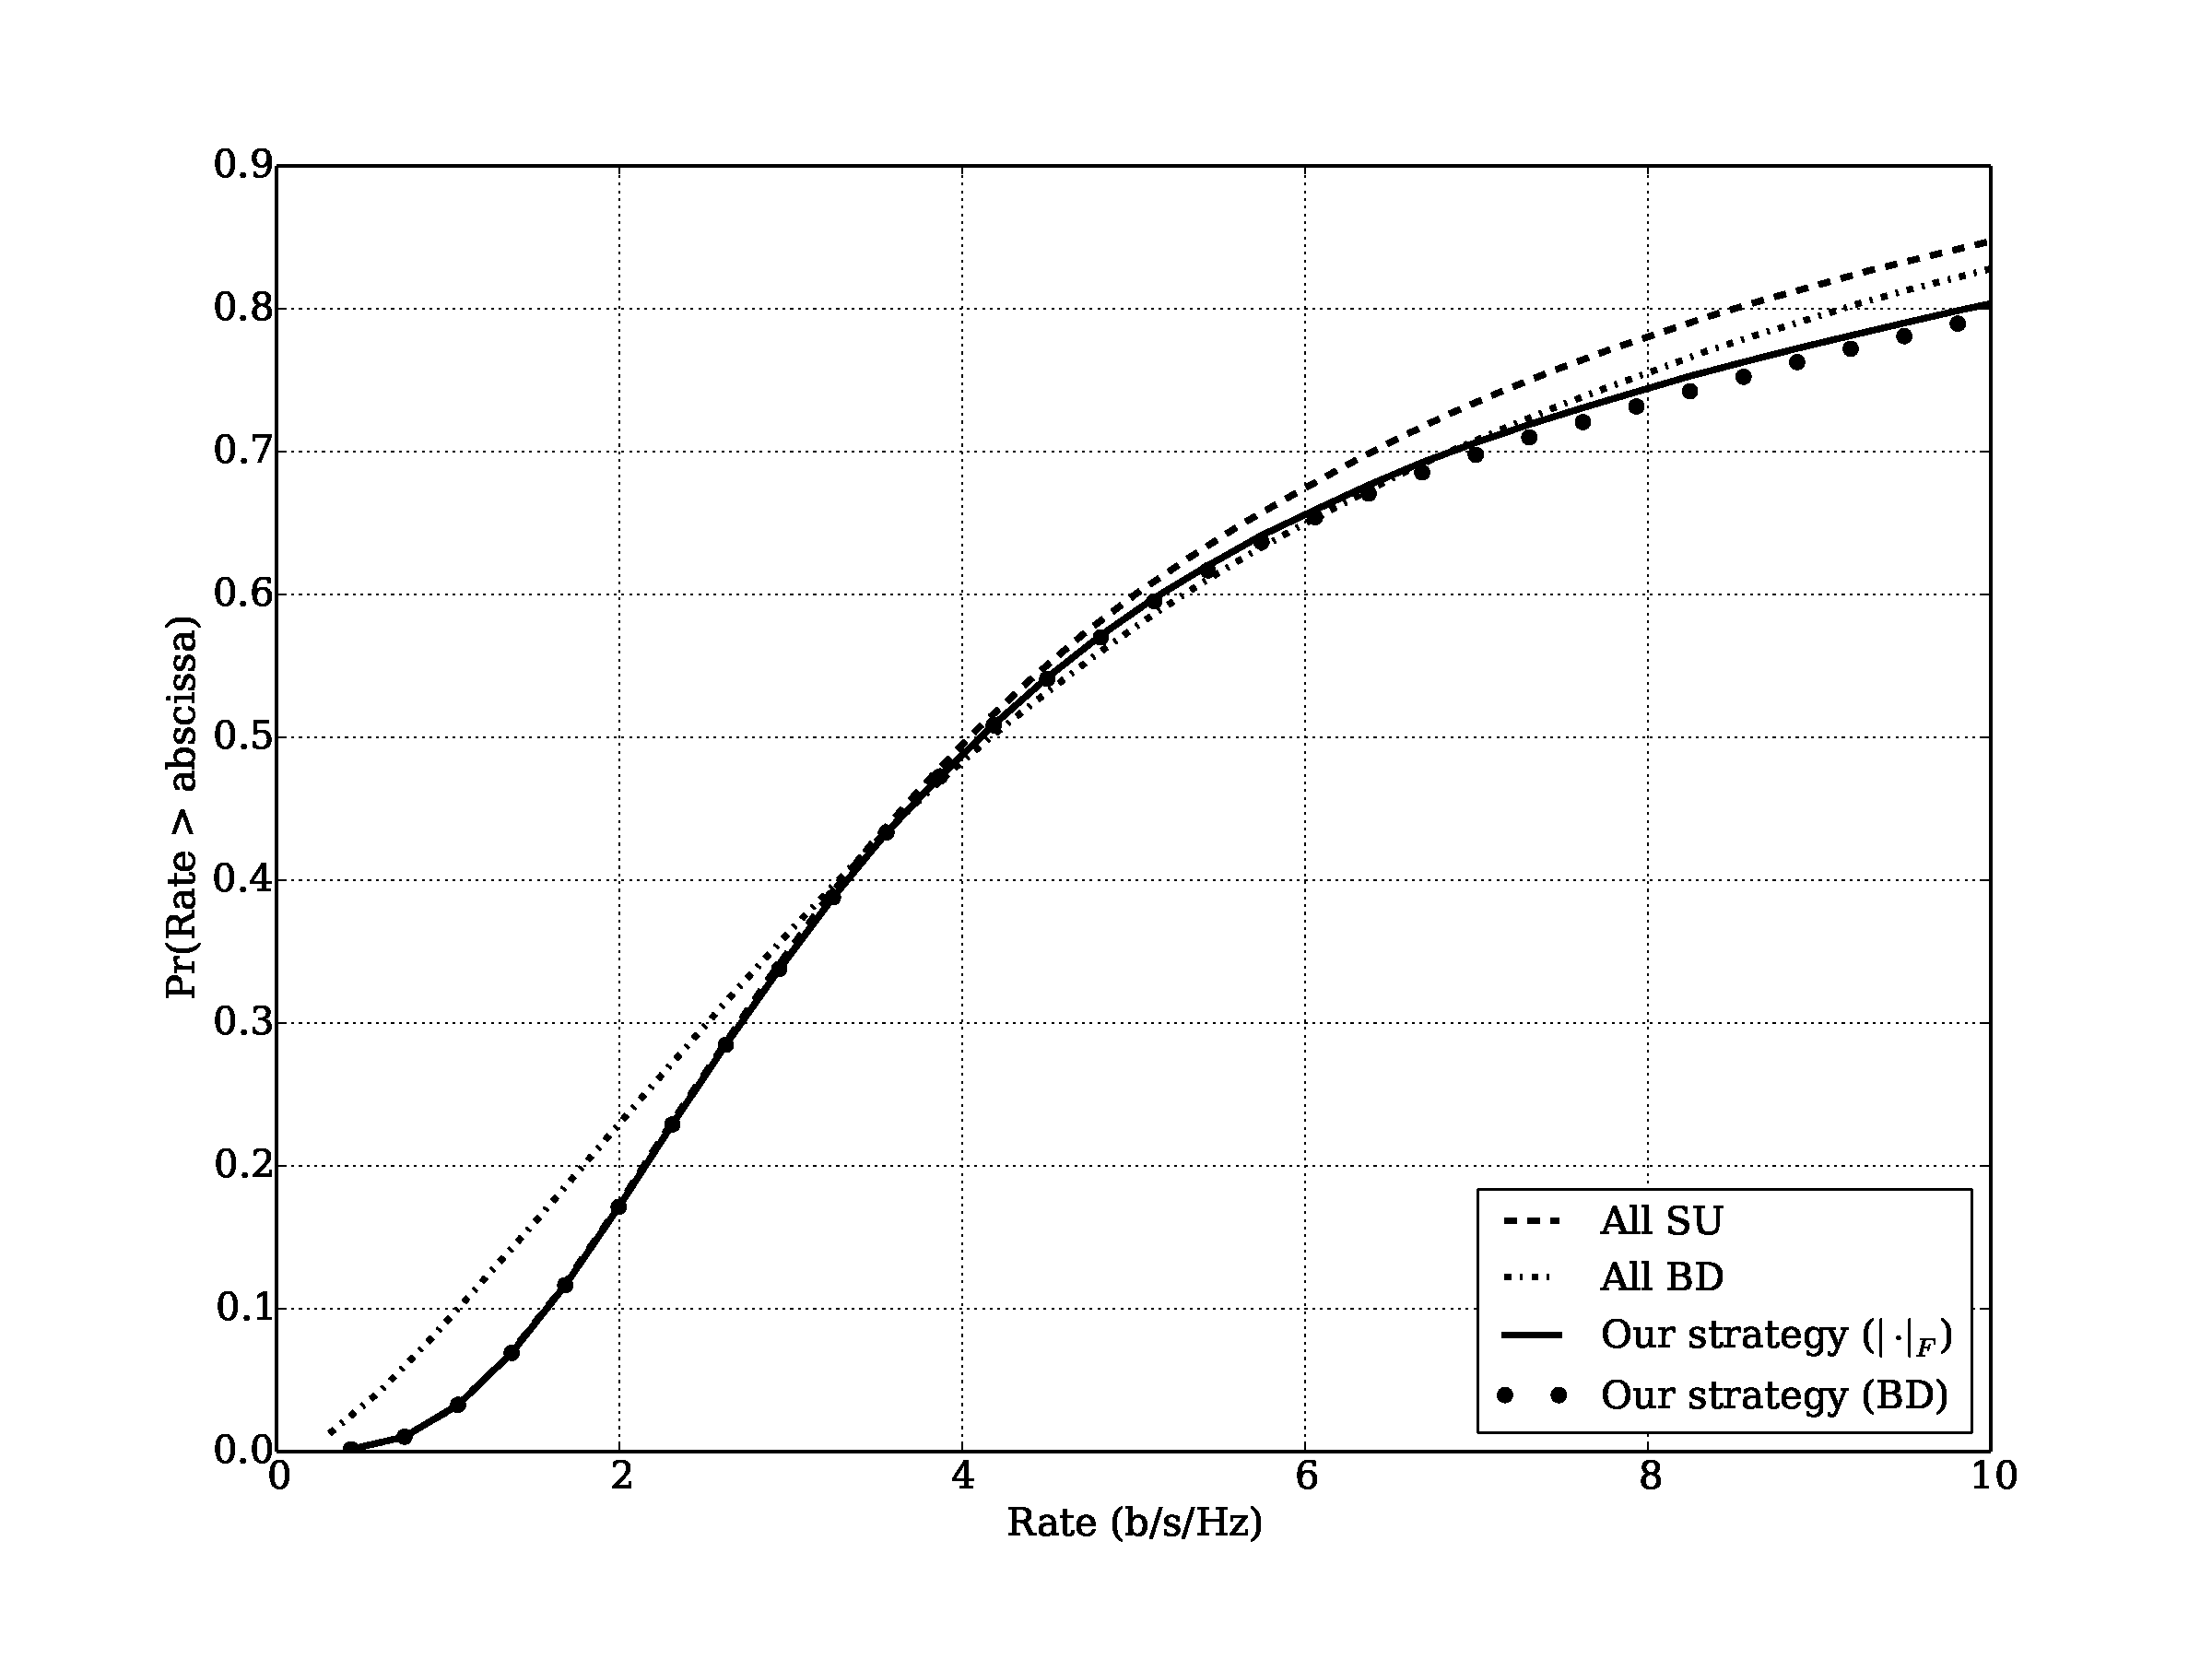
\includegraphics[width=0.75\columnwidth]{./12.simple_threshold_scheduling/img/cdf_02x02_s20_100user_bd} \caption{CDF of the rates obtained in a 2x2 scenario, with an SNR of $10$\,dB.}
\label{fig:cdf_snr10}
\end{figure}

\begin{figure}[t]
\centering
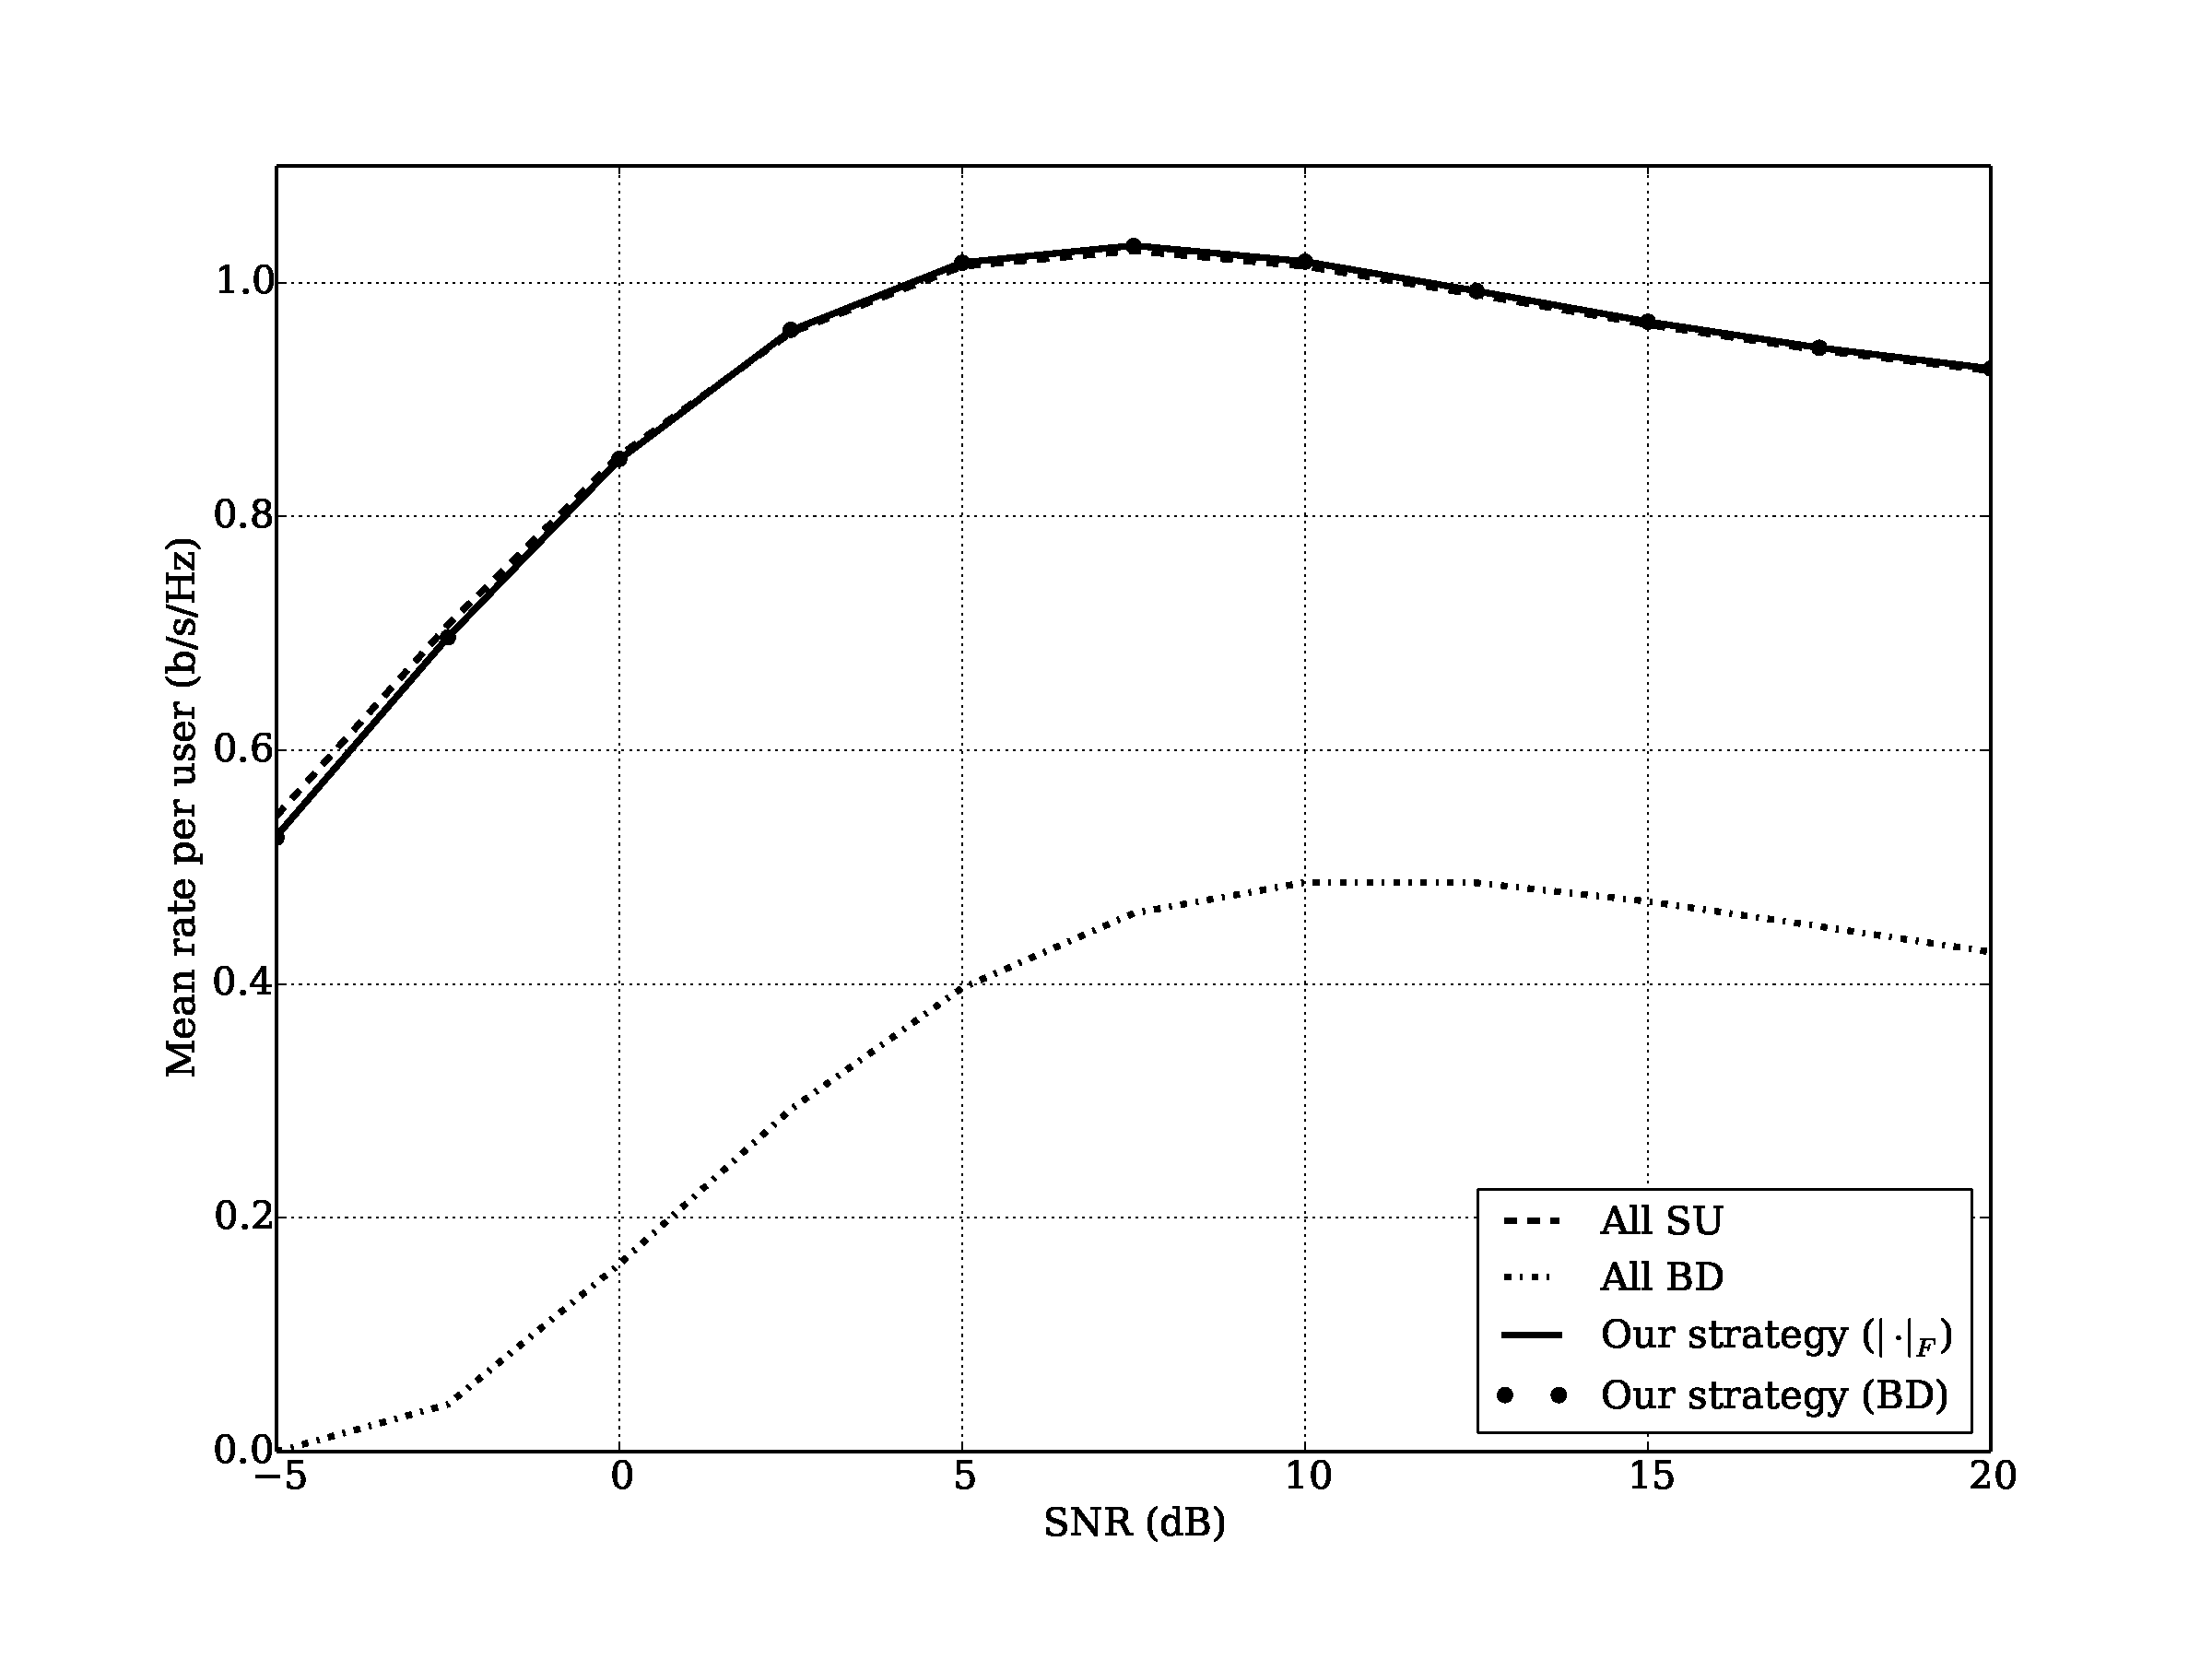
\includegraphics[width=0.75\columnwidth]{./12.simple_threshold_scheduling/img/mean_rate_005_worst_02x02_100user_bd} \caption{Mean rate of the 5\% worst users, in a 2x2 scenario in the presence of OCI, 100 users per cell.}
\label{fig:worst_rate}
\end{figure}
